\section{Learning from Demonstration}
In this research, we proposed a framework that enables the robot to learn new motions by observing human demonstrations. The learning process consists of two phases. The first is the observation phase, where the robot observes the demonstrations performed by the human and acquires sample trajectories for the tasks. The second phase is the modification phase, where the robot tries to reproduce the tasks by following the observed trajectories. During the reproduction, the human can correct and modify the robot's motions and update the trajectories.

\subsection{Observing Human Demonstration}
If there is an operation target object, the trajectory should be recognized as the one relative to the target object. In such a case, once the coordinates of the target object are recognized, the trajectory of the hand in a human performance can be converted into the one relative to the target with the following equation.
\def\vector#1{\mbox{\boldmath $#1$}}
\begin{align}
  ^{ref}\!\vector{x}_{target} &= H_{ref}^T \vector{x}_{demo} \\
  where \ \
  ^{**}\!\vector{x}_{*} &= \left(
  \begin{array}{cc}
    ^{**}\!\vector{p}_{*}^{T} & 1
  \end{array}
  \right)^T \nonumber
\end{align}
where \(\vector{p}_{demo}\) is the position of the hand in the human demonstration and \(^{ref}\!\vector{p}_{target}\) is the converted position, which the robot remembers. \(H_{ref}\) is the homogeneous transformation matrix from the absolute coordinates to the reference target coordinates.

\subsection{Reproducing according to Demonstration}
To decide the robot motion, the robot needs to know a pair of the target position and the target orientation in each time step. A set of target positions, the trajectory, can be acquired by observing the human demonstration. We introduced the idea to use the potential field and decide the desired orientation in each target position.
\subsubsection{Using Potential Field with PointCloud}
We extended the use of the potential field to PointCloud. The potential field in each position \(\vector{r}\) can be computed as following.
\begin{equation}
  \label{equation:electronic_potential_pointcloud}
  \vector{E}(\vector{r}) = - {\sum_{\vector{p} \in PC} { \frac {\vector{r} - \vector{r'}(\vector{p})} {\| \vector{r} - \vector{r'}(\vector{p}) \| ^ 3} } }
\end{equation}
where \(\vector{r'}(\vector{p})\) is the position of each PointCloud. Figures below illustrate the examples of the potential field around a table and a kitchen.

\vspace{-3mm}
\begin{figure}[htbp]
  \begin{center}
    \begin{minipage}{0.45\hsize}
      \begin{center}
        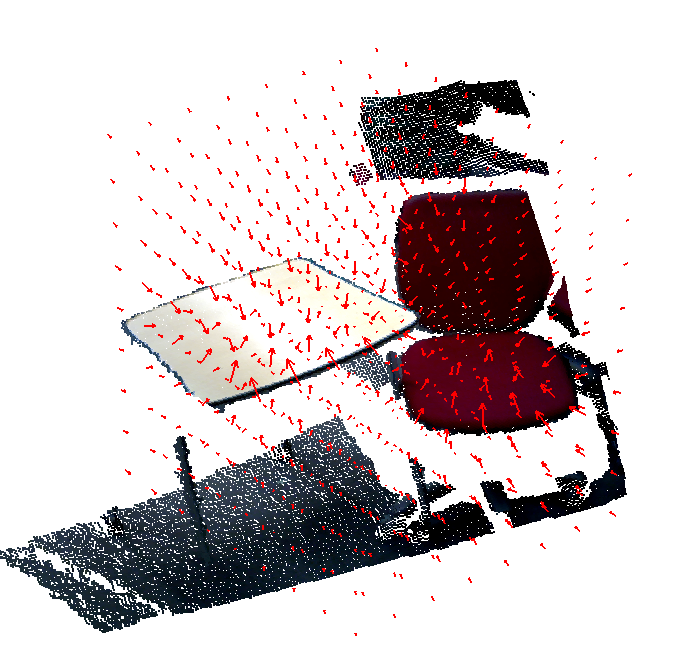
\includegraphics[clip, width=1.0\columnwidth]{figs/table-chair-potential.png}
        \label{figure:table_potential}
      \end{center}
    \end{minipage}
    \begin{minipage}{0.45\hsize}
      \begin{center}
        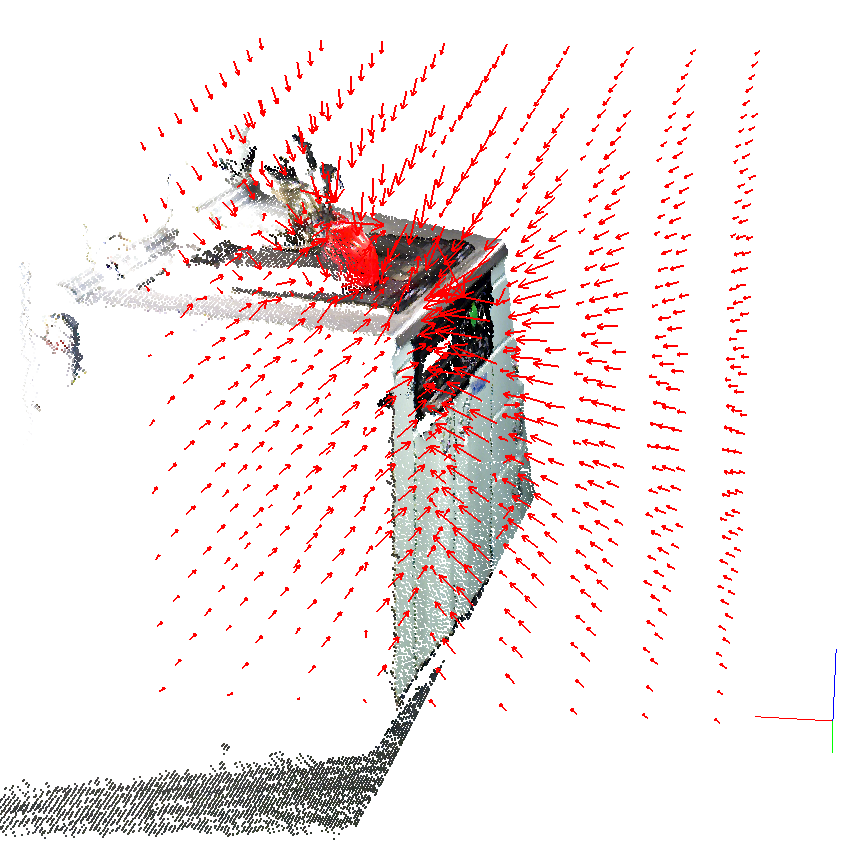
\includegraphics[clip, width=0.9\columnwidth]{figs/kitchen_potential_side_3.png}
        \label{figure:kitchen_potential}
      \end{center}
    \end{minipage}
  \end{center}
  \vspace{-3mm}
  \caption{\footnotesize{Examples of the potential field with the PointCloud around a table and a chair (left), and a kitchen (right).}}
  \vspace{-3mm}
\end{figure}

The orientation in each position can be computed with \equref{electronic_potential_pointcloud}, and finally the robot posture can be computed with solving the Inverse Kinematics with the target coordinates defined by this pair of the potision and the orientation.

\subsubsection{Enabling Other Moving Targets besides Hands}
We also improved our system so that other moving targets are available. We use our finger to press a button, or we consider the working point to use a certain tool. To plan those things for a robot, we suppose new coordinates that represent those working point. The robot can solve the Inverse Kinematics with those new coordinates and get a desired posture through the same procedure with hands.
\begin{figure}[htbp]
 \begin{center}
  %% \includegraphics[width=1.00\columnwidth]{figs/move-targets}
   \begin{minipage}{0.30\hsize}
     \begin{center}
       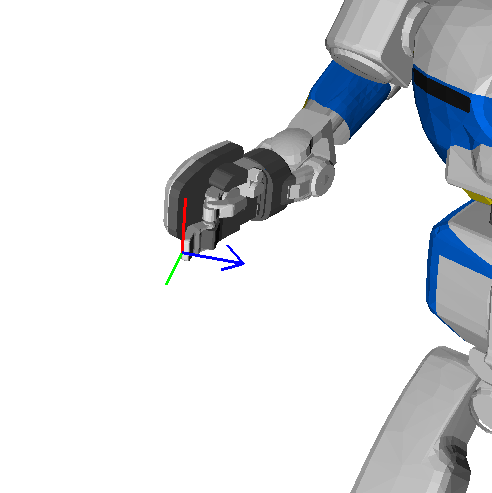
\includegraphics[clip, width=1.0\columnwidth]{figs/finger-move-target.png}
     \end{center}
   \end{minipage}
   \begin{minipage}{0.30\hsize}
     \begin{center}
       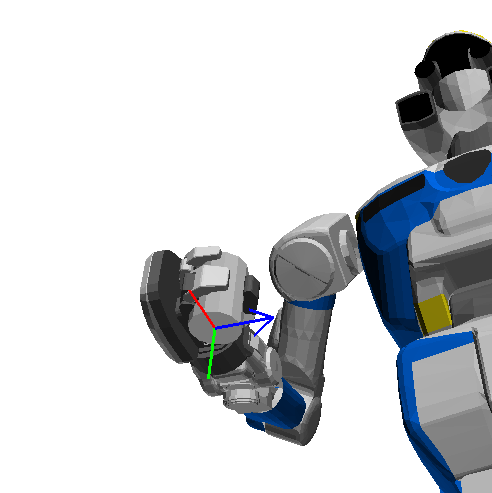
\includegraphics[clip, width=1.0\columnwidth]{figs/hanko-move-target.png}
     \end{center}
   \end{minipage}
   \begin{minipage}{0.30\hsize}
     \begin{center}
       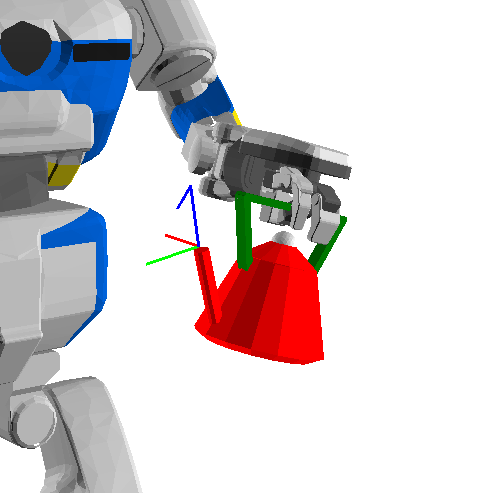
\includegraphics[clip, width=1.0\columnwidth]{figs/kettle-move-target.png}
     \end{center}
   \end{minipage}
  %% \vspace{-2mm}
  \caption{\small{Other moving targets besides hands. Figure show exaples with a finger, a stamp and a kettle.}}
  \label{figure:move_target}
 \end{center}
 \vspace{-8mm}
\end{figure}

\begin{table*}[htbp]
  \begin{center}
    \vspace{-7mm}
    \caption{\small{A sample speech flow during the teaching and the labelling phases}}
    \vspace{-2mm}
    \footnotesize
    \begin{tabular}{|c|c|l|l|} \hline
      \# & Human/Robot & Speech & Sample code\\ \hline\hline
      1 & Human & I'll teach you how to {\bf push the stove button}. & set motion-name to ``push the stove button''\\
      2 & Robot & Okay, is there an operation target? &\\
      3 & Human & {\bf button.} & insert \{target : ``button''\} to motion-info \\
      4 & Robot & Is there anything to move? &\\
      5 & Human & {\bf Your finger.} & insert \{move-target : ``finger''\} to motion-info\\
      6 & Robot & I'll be looking at you, so please start with saying ``Start.'' &\\
      7 & Human & Start. ...(demonstration)... Finished. & insert \{target-position-list : demonstration-data\} to motion-info\\
      8 & Robot & I remembered {\bf push the stove button} motion. & insert \{motion-name : motion-info\} to motion-table\\ \hline\hline
      9 & - & (the kettle whistles) &\\
      10 & Human & Listen to this sound. &\\
      11 & Robot & Okay, I'll listen. ...(listen) & set sound-feature to {\sl unique-freq}\\
      12 & Robot & I've heared clearly. What's this sound? &\\
      13 & Human & It's the sound of {\bf kettle}. & set ``kettle'' to sound-name\\
      14 & Human & Okay, I remembered. & insert \{sound-name : sound-feature\} to sound-table\\ \hline\hline
      15 & Human & When you hear the sound of a {\bf kettle}, please {\bf push the stove button}. & insert \{``kettle'' : ``push the stove button''\} to condition-table\\ \hline
    \end{tabular}
    \label{table:speech_flow}
  \end{center}
  \vspace{-6mm}
\end{table*}

\subsection{Modifying Trajectory}
The rough plan for the robot is acquired from the human demonstration. However, the first plan is likely to be wrong. The reasons for this failuare might be visual errors during the observation phase or conflictions with other control systems like stabilization. To correct these errors, the human can grab the robot's hand and modify the planned trajectory interactively utilizing the force sensors on the wrists and the ankles.

%% \begin{algorithm}
%%   \footnotesize
%%   \caption{Target position updater}
%%   \begin{algorithmic}
%%     \STATE $\vector{d} \leftarrow (
%%     \begin{array}{ccc}
%%       0 & 0 & 0
%%     \end{array}
%%     )^\top$
%%     \FOR{$\vector{x}_{target, t}$ in X}
%%     \STATE $\vector{x}_{target, t} \leftarrow \vector{x}_{target, t} + \vector{d}$
%%     \IF{$\|\vector{f}_t\| > f_{thre}$}
%%     \STATE $\vector{d} \leftarrow \vector{d} + \alpha \vector{f}_t$
%%     \ENDIF
%%     \ENDFOR
%%     %% \ENDWHILE
%%   \end{algorithmic}
%% \end{algorithm}

%% \begin{figure}[htbp]
%%   \begin{center}
%%     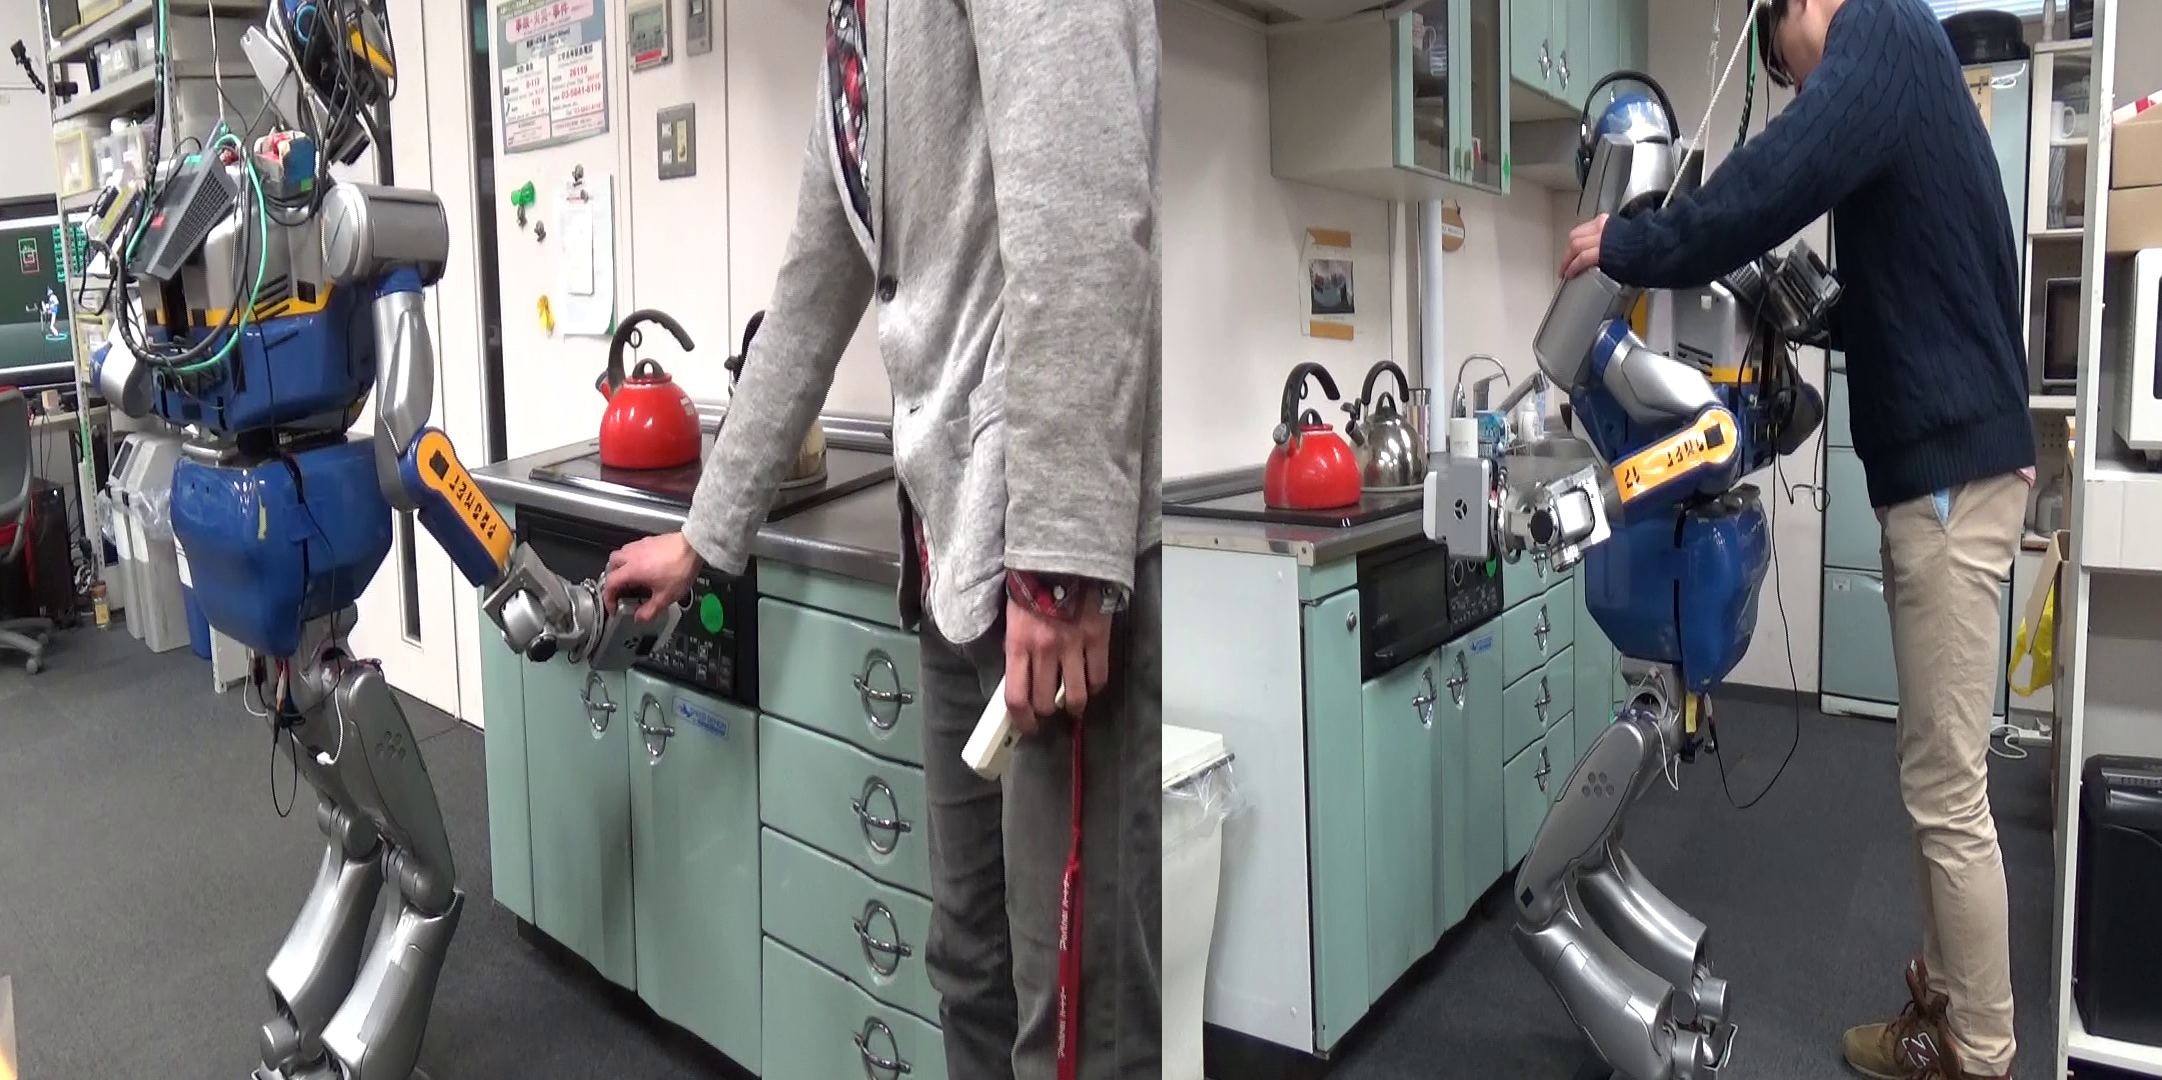
\includegraphics[clip, width=0.8\columnwidth]{figs/modify.png}
%%     \label{figure:modification_trajectory}
%%   \end{center}
%%   \caption{\footnotesize{}}
%% \end{figure}
